% Gemini theme
\documentclass[final]{beamer}

% ====================
% Packages
% ====================

\usepackage[T1]{fontenc}
\usepackage{lmodern}
\usepackage[size=custom,width=120,height=90,scale=1.0]{beamerposter}
\usetheme{gemini}
\usecolortheme{gemini}
\usepackage{graphicx}
\usepackage{booktabs}
\usepackage{tikz}
\usepackage{pgfplots}
\usepackage{verbatim}
\usepackage{framed}

% ====================
% Lengths
% ====================

% If you have N columns, choose \sepwidth and \colwidth such that
% (N+1)*\sepwidth + N*\colwidth = \paperwidth
\newlength{\sepwidth}
\newlength{\colwidth}
\setlength{\sepwidth}{0.025\paperwidth}
\setlength{\colwidth}{0.3\paperwidth}

\newcommand{\separatorcolumn}{\begin{column}{\sepwidth}\end{column}}

% ====================
% Title
% ====================
\title{Analyzing and Estimating Cyberattack Trend by Performing Data Mining on Cybersecurity Data Set}

\author{Chan Young Koh}

\institute{Bridgewater State University\samelineand(Mentor: Dr. Enping Li)}

% ====================
% Body
% ====================

\begin{document}

\begin{frame}[t]
\begin{columns}[t]
\separatorcolumn

% Objective 
\begin{column}{\colwidth}

  \begin{block}{Main Objective}
  
    \begin{itemize}
        
  
        \item Data mining is the process of finding anomalies, patterns, and correlations within a large data set to predict the outcome. 
        
        \item R is a language and environment for statistical computing and graphics. With R, we were able to parse relatively large data to extract meaningful pattern, which will be used to determine the future trend. 
        
        \item This research focuses on finding the future trend of cyberthreats through data mining using R. Once we discover a reasonable trend, we will provide countermeasures regarding a group of most notorious cyberthreats. 
    
    \end{itemize}

  \end{block}

  \begin{block}{Motivation}
% brief introduction on why it is important 
% state motivation on why this research is important 
% Available countermeasures people can apply 
% Each particular attack, attach image to denote the attack.

    \begin{itemize}
        \item Damage related to cybercrime is expected to hit 6 trillion USD annually by the year of 2021. 
        \item More than five (5) billion accounts were compromised within three years (2016-2018). 
        \item Countless cyberthreats are discovered daily, and it is important for the public to be aware of the gravity of cyberattacks. 
    \end{itemize}

   

  \end{block}
  
  \begin{block}{Dataset}
    \begin{itemize}
        \item Three datasets that contain cyberthreat records from 2016 to 2018 respectively.
        \item Each dataset was separated into months. Utilization of R allowed us to combine datasets into three annual datasets. 
        \item Some of the entries had "unknown" as their values. Hence, to reduce ambiguity, we have removed rows that contain "unknown" data. 
        \item Apart from the data containing "unknown", we also discovered few outliers in the data. Thus, we have removed them from consideration since outliers barely affect the trend of the data. 
    \end{itemize}
  \end{block}
  

  \begin{alertblock}{Terminology}
  
  % add another block regarding why I chose the dataset, and how I parsed it. 
   
        

    \begin{itemize}
      \item \textbf{Account Hijacking}: The process through which any person's or organization's account(s)- be their email, social media or other accounts - is/are stolen or hijacked by a hacker. 
      \item \textbf{Malware}: Malware is short for "malicious software" - computer programs designed to infiltrate and damage computers without the users consent. 
      \item \textbf{PoS Malware}: Point-of-Sale malware targets consumers' personal and financial data stored on either credit or debit cards. Hacker will hack the Point-of-Sale machine and use RAM scrapers to collect and sell customer information. 
      \item \textbf{DNS Hijacking}: Domain Name Server Hijacking, also known as DNS redirection, is a type of DNS attack in which DNS queries are incorrectly resolved in order to unexpectedly redirect users to malicious websites. 
      \item \textbf{SQL Injection}: SQL Injection or SQLi is a type of database threats, in which an attacker uses webpages to plant the attack. Hackers would include malicious SQL query statements in the web server. One loophole in the server may send these malicious SQL query statements into the database itself, causing a deletion of entire database or a severe malfunction. 
      \item \textbf{Privilege Escalation}: Privilege Escalation is a database threat where a hacker usually injects script in order to find out most generous level of privileges in a database server. Once the hacker detects the best privilege in the server, the hacker will abuse the privilege to create further damage. 
      \item \textbf{Whitelist}: A whitelist is a cybersecurity list, only giving administrator-approved programs, and IP and email address, system assess. Any information not on the list will blocked. 
      \item \textbf{Multi-factor Authentication}: An authentication method which grants access to a computer user after the user successfully presents two or more validation components. 
      \item \textbf{Targeted Attack}: A type of cyberthreat in which perpetrators actively pursue and compromise a target entity's infrastructure while maintaining anonymity. These attackers have a certain level of expertise and have sufficient resources to conduct their schemes over a long-term period. They can adapt, adjust, or improve their attacks to counter their victim's defenses. 
      \item \textbf{Privileged Access Workstation}: A Privileged Access Workstation (PAW) is a dedicated computing environment for sensitive tasks that is protected from Internet attacks and other threat vectors. A PAW separates these sensitive task and accounts from non-administrative computer use, such as email and web browsing.
      \begin{figure}[h!]
        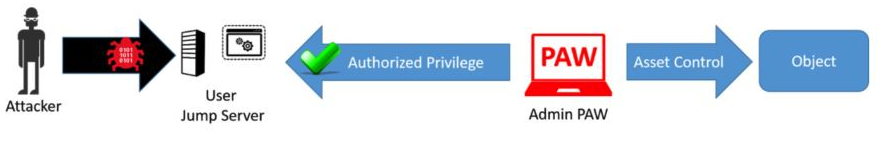
\includegraphics[width=0.67\textwidth]{PAW.png}
        \caption{A use case diagram of one of PAW models.}
      \end{figure}
    \end{itemize}

   

  \end{alertblock}
  
  

\end{column}




\separatorcolumn
%Use \begin{enumerate} to start numbered list 
\begin{column}{\colwidth}

  \begin{block}{Cyberattacks Statistics}
  % Mention about why I chose this dataset. 
      
  
    \frame{\resizebox{.5\textwidth}{.15\textheight}{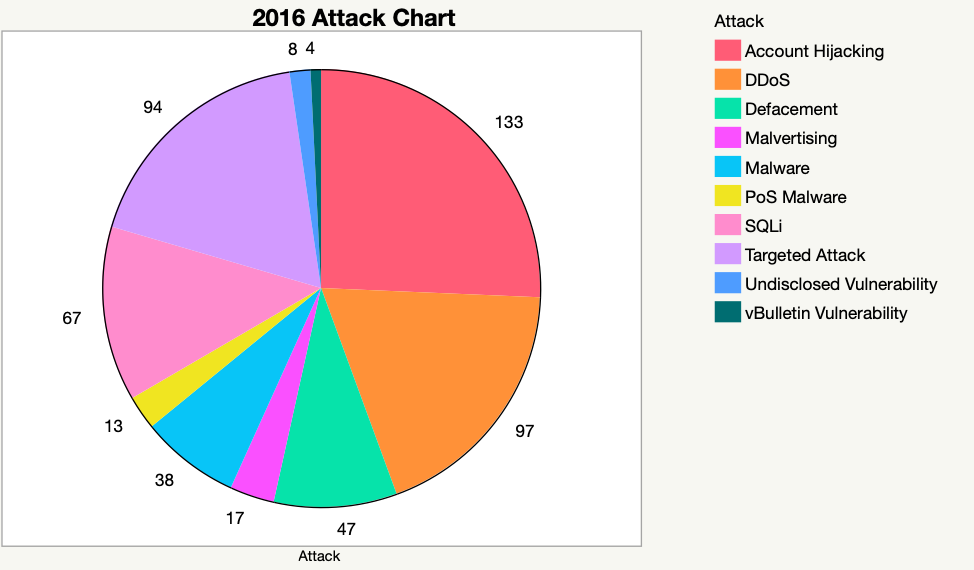
\includegraphics{2016data.png}}}
    \frame{\resizebox{.5\textwidth}{.15\textheight}{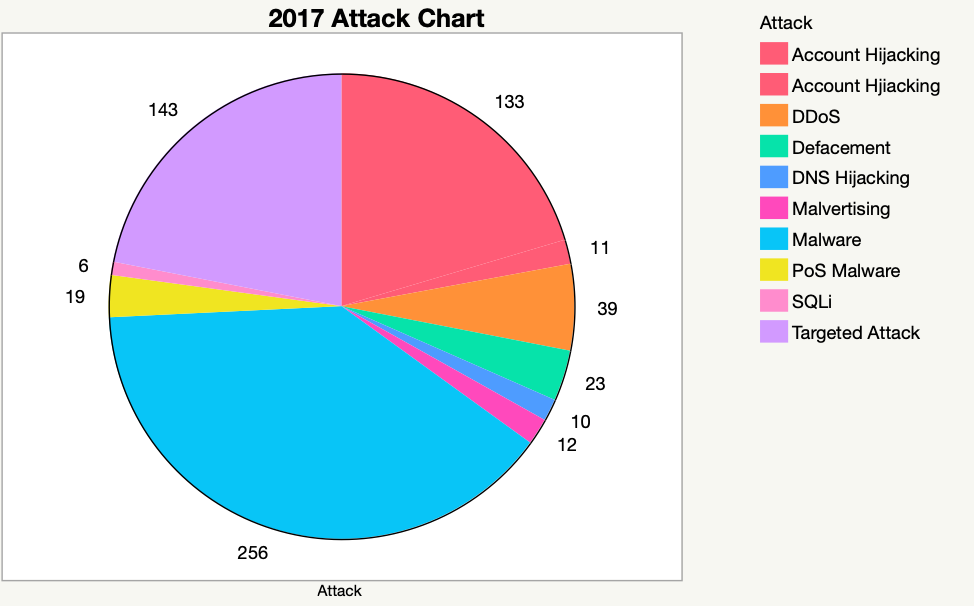
\includegraphics{2017data.png}}}
    
    \begin{center}
        \frame{\resizebox{.5\textwidth}{.15\textheight}{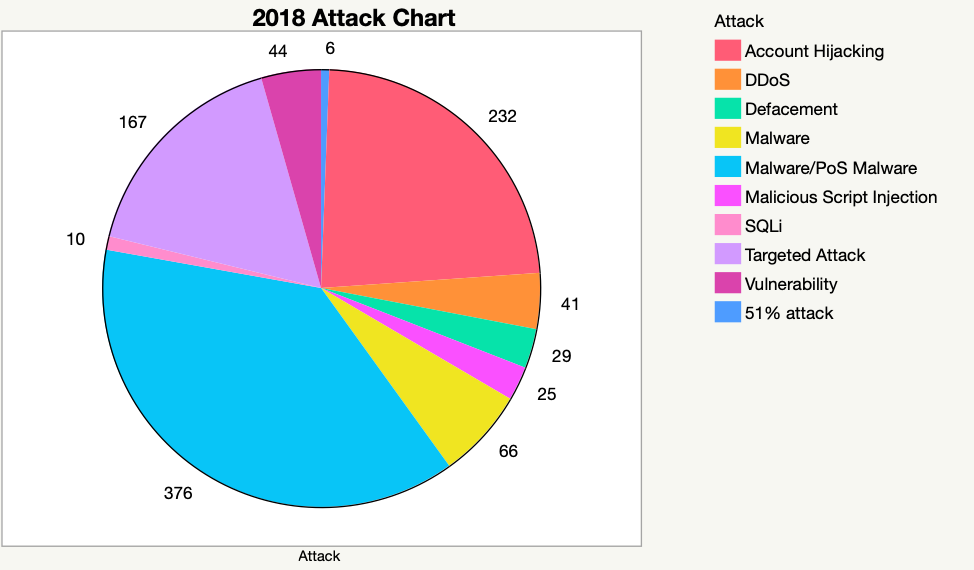
\includegraphics{2018data.png}}}
    \end{center}%\frame{\resizebox{.33\textwidth}{.1\textheight}{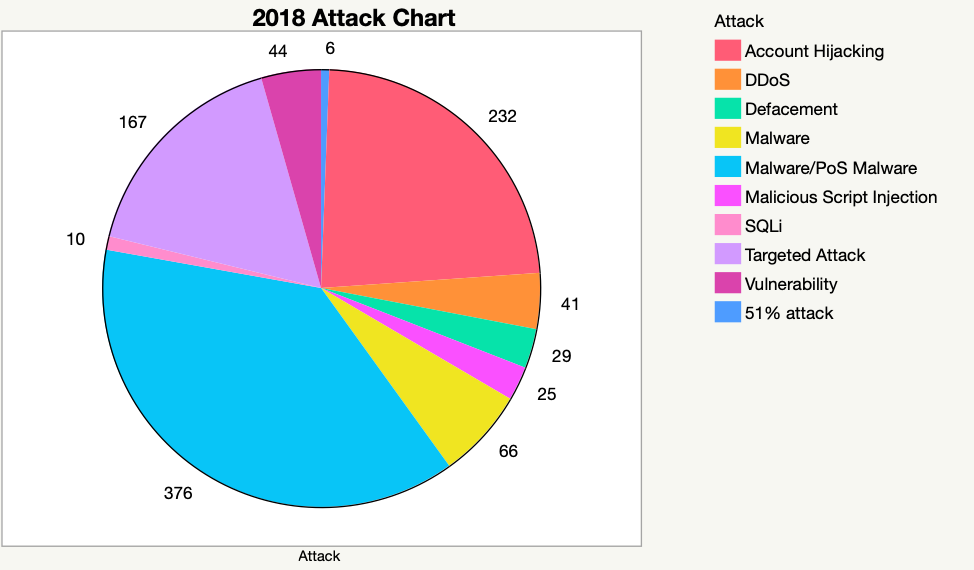
\includegraphics{2018data.png}}}
    
    \begin{itemize}
        \item Account Hijacking maintained an average of 23.13\% of major cybercrimes which occurred in three years. 
        \item The number of cybercrimes related to malwares has increased by \textbf{866.7\%} since 2016. 
        \item The number of targeted cyberattacks has increased by 18\% since 2016. 
        \item A burst of SQL Injection attacks happened in 2016 which targeted the Board of Elections. In summer 2016, voter data of 200,000 citizens were hacked by hackers through SQLi. 
        \item On October 21, 2016, a series of \textit{distributed denial-of-service attacks} occurred. This series of DDoS attacks was aimed at Domain Name System(DNS) provider named \textbf{Dyn}. More than 30 prestigious companies were affected by this attack until they found a remedy after almost 12 hours. 
    \end{itemize}

      

    %\begin{itemize}
       
      %\item \textbf{figure 1 }, suggests summary of cyberattacks during the entire year of 2016. Five most notorious threats were Account Hijacking, Targeted Attack, Defacement, Malvertizing, and Undisclosed Vulnerability respectively. 
    %\end{itemize}

  \end{block}

  \begin{block}{Countermeasure}
% Pie chart along with counter measures 
   Discuss countermeasures

   %
\includegraphics[width=1\linewidth]{placeholder}

  \end{block}

 

\end{column}

\separatorcolumn

\begin{column}{\colwidth}

  \begin{block}{Countermeasure Part II}

    Include more countermeasures 

 

    \heading{Countermeasure #1}

    Explain

    \heading{Countermeasure #n}

    Explain
  \end{block}

  \begin{block}{Future Research Development}

    I would like to portrait what I would want to research more about after this research. Will I continue? If so, how would I continue? 

    %\begin{table}
     % \centering
      %\begin{tabular}{l r r c}
       % \toprule
        %\textbf{First column} & \textbf{Second column} & \textbf{Third column} & %\textbf{Fourth} \\
        %\midrule
        %Foo & 13.37 & 384,394 & $\alpha$ \\
        %Bar & 2.17 & 1,392 & $\beta$ \\
        %Baz & 3.14 & 83,742 & $\delta$ \\
        %Qux & 7.59 & 974 & $\gamma$ \\
        %\bottomrule
      %\end{tabular}
      %\caption{A table caption.}
    %\end{table}


    

  \end{block}

  \begin{block}{References}

    \nocite{*}
    \footnotesize{\bibliographystyle{plain}\bibliography{poster}}

  \end{block}

\end{column}

\separatorcolumn
\end{columns}
\end{frame}

\end{document}
